\section{Experiment}
% 为了验证本文方法及工具的可行性与正确性,本章给出了对布尔程序逆向转换修复的测试实验。
To verify the effectiveness and correctness of the methods and tool described in former sections, detailed experimental results and analysis will be given in this following section.
% 本章实验通过对现有的标准程序进行修复和转换,从修复结果的准确率和修复的效率等方面对布尔程序逆向转换工具进行评价
In the experiment, the program repair tool will be used to repair some programs and evaluated based on its accuracy and efficiency.

% 在本章的实验中,主要针对工具能够修复的赋值错误和控制条件语句错误进行了修复及转换测试
The experiment mainly tested the tool on its ability to convert and repair assignment statements and conditional control flow statements (\lstinline|if|).
% 其中选取了在程序诊断中比较常用到的西门子套件中的TCAS程序以及一些针对TCAS未能覆盖的循环语句条件错误的测试程序。
To be more specific, Several test cases of TCAS program from Siemens Suite, which has been used as a benchmark to evaluate the effectiveness of many testing techniques, are used in this experiment. More customized programs are added to the test cases to test the tool's ability of repairing boolean expression faults in loop statements, which Siemens' TCAS fails to cover.

\subsection{TCAS of Siemens Suite}
\subsubsection{Introduction}
% TCAS程序是程序诊断的基准测试用例集西门子套件中的其中一个程序,
The TCAS program used in the experiment comes from Siemens Suite, which has been used by other recent works on fault localization\cite{EotEoDaCBTAC,ESoaRTST}.
% 该程序的主要功能是模拟飞机调度中产生冲突的情况及给出了防止飞机相撞的办法。[51]
TCAS, or traffic collision avoidance system, is an aircraft collision avoidance system designed to reduce the incidence of mid-air collisions between aircraft\cite{TCAS}.
% TCAS有正确版本的程序以及41个不同错误版本的错误程序,此外,在TCAS的基准套件中还给出了1608个不同的测试用例输入。
Siemens Suite provides a correct TCAS program, along with 41 different faulty versions. Additionally, 1608 different test cases are provided in Siemens Suite.
% 程序长度为173行,包含25个全局变量,除main函数外还有其他8个函数,因此程序中有函数调用。
The program has 173 lines of statements, including 25 global variables and 8 functions except for \lstinline|main| function.
% 在给出的41个不同错误版本中,V10、V11、V15、V31、V32、V33、V40的版本中包含多个错误,不在本文的修复考虑行列,因此不做统计。
Among the 41 given faulty versions, $V10$, $V11$, $V11$, $V15$, $V31$, $V31$, $V32$, $V33$, $V40$ contain multiple faults in one file, which is not supported by the tool, hence they will not be considered in the experiment.
% 表5-1给出对了TCAS程序的其余34个错误版本的错误类型统计,其中修复错误归类为赋值语句右部错误以及控制条件语句错误的版本为本文能够修复的错误。
The statistics of the rest 34 versions is listed in table \ref{table:SoTCASTC}, in which assignment statement fault and conditional control flow statement fault are supported by the tool.

\begin{table}
\small
\center
\caption{Statistics of TCAS Test Cases}
\label{table:SoTCASTC}
\begin{tabular}{lll}
\hline
Version                                 & Fault Type                  & Detailed Fault Type         \\
\hline
$5$,$21$,$22$,$23$,$24$,$27$,$41$       & Assignment Statement Fault  & Logical Error in Assignment \\
$1$,$3$,$4$,$6$,$9$,$12$,$20$,$25$,$39$ & Assignment Statement Fault  & Wrong Operator              \\
$13$,$14$,$16$,$17$,$18$,$19$,$36$,$38$ & Declaration Error           & Declaration Error           \\
$2$,$28$,$29$,$30$,$35$,$37$            & Assignment Statement Fault  & Wrong `return` Statement    \\
$7$,$8$                                 & Assignment Statement Fault  & Initialization Error        \\
$34$                                    & Conditional Statement Fault & Wrong Condition Expression  \\
\hline
\end{tabular}
\end{table}

\subsubsection{Preprocess on Test Cases}
% TCAS程序在运行的时候需要读取参数作为输入,但是本修复工具在C程序转换为布尔程序的过程中,C程序已经包含了测试用例,即程序的输入和输出已经加进了C程序之后才将其转换为布尔程序。
To execute the TCAS program, designated input is needed, but the repair tool we design assumes the given $C$ program already includes test case.
% 因此针对每个错误版本的C程序,首先将选定的一个或多个测试用例直接赋给相关需要读入参数的变量,并且将预期输出结果以”assert(output ==  expected)"的形式加在main函数返回语句之前。
In this case, for each faulty version, one or more test cases will be selected to assign to the respective input variables, while new \lstinline|assert| statement will be added just before the end of \lstinline|main| function
to examine the program's output.
% 程序在加入测试用例的输入和预期输出后则表示给出了程序的行为规范,assert语句规定了程序的正确终止状态,因此如果在模拟函数运行的过程中路径到达的状态不满足当前的assert语句,则表示到达的是错误终止状态,即该路径是错误路径。
By doing so, the given input and expected output of the test cases give out the specification of the program's behavior.

% 在对TCAS的修复实验中,为了验证前文提到的多个测试用例修复方法还进行了当程序只加入一个测试用例输入以及加入多个测试用例输入时的结果对比。
In the TCAS repairing experiment, we introduced different numbers of test cases to one faulty version, hoping to prove the effectiveness of the multi-test-case repair method we described in section \ref{section:MultipleTestCasesRepair}.

\subsubsection{Experimental Results}
% 针对表5-1中可以被修复的26个程序版本进行了实验,对于这些版本的错误, 使用多个测例进行修复并转换的方法均能找到程序的修复。
We experimented on the 26 faulty versions listed in table \ref{table:SoTCASTC} whose faults are supported by the tool. For the faults of these versions, the repairing method which uses multiple test cases managed to locate all of them.

% 表5-2列举了其中10个版本的程序的测试实验结果。
% TODO 加入表格引用
The results of 10 of them are listed in table \ref{table:RoTCASTC}. Meanings of columns in table \ref{table:RoTCASTC} are listed below:

\begin{enumerate}
\item {\it Version}   : the version number.
\item $V$             : the number of global and relevant boolean variables.
\item $LoBP_{1}$      : the length of converted boolean program when only one test case is introduced.
\item $Time_{1}$($s$) : the time in seconds used to repair the given boolean program when only one test case is introduced.
\item $Result_{1}$    : the percentage of passed tests among the given 1608 tests when only one test case is introduced.
\item $LoBP_{2}$      : the length of converted boolean program when multiple test cases are introduced.
\item $Time_{2}$($s$) : the time in seconds used to repair the given boolean program when multiple test cases are introduced.
\item $Result_{2}$    : the number of test cases which cover bad routes effectively and the number of test cases we use.
\end{enumerate}

We shall give you a detailed insight into one of them. Takes $V1$ as an example, we used 6 test cases to find out a correct repair statement, which was $*rep=(b4)|(b3)|(b2)|(!b1)|(b0)$ with respective predicates of each variable listed below:

\begin{itemize}
\item[-] $\text{b0} : \textit{Down\_Separation} - \textit{Positive\_RA\_Alt\_Thresh}[\textit{Alt\_Layer\_Value}] == 0$
\item[-] $\text{b1} : \textit{Down\_Separation} - \textit{Positive\_RA\_Alt\_Thresh}[\textit{Alt\_Layer\_Value}] <= 0$
\item[-] $\text{b2} : \textit{Other\_Tracked\_Alt} - \textit{Own\_Tracked\_Alt} <= 0$
\item[-] $\text{b3} : \textit{Down\_Separation} - \textit{Positive\_RA\_Alt\_Thresh}[\textit{Alt\_Layer\_Value}] >= 0$
\item[-] $\text{b4} : \textit{Down\_Separation} - \textit{Up\_Separation} >= 100$
\end{itemize}

Judging from the experimental result, $*rep$ is satisfiable. After applying the simplification rules we described in former section, we have a converted $C$ repair statement \lstinline|Down_Separation - Positive_RA_Alt_Thresh[Alt_Layer_Value] < 0| \lstinline| && | \lstinline|Down_Separation - Up_Separation < 100| \lstinline| && | \lstinline|Other_Tracked_Alt - Own_Tracked_Alt > 0|. After replacing the faulty statement with the above statement, the repaired program passed all test cases.

\begin{table}
\small
\center
\caption{Results of TCAS Test Cases}
\label{table:RoTCASTC}
\begin{tabular}{|c|c|c|c|c|c|c|c|}
\hline
Version & $V$     & $LoBP_{1}$ & $Time_{1}$($s$) & $Result_{1}$ &$LoBP_{2}$ & $Time_{2}$($s$) & $Result_{2}$ \\
\hline
$1$     & $6/22$  & $806$      & $66.6$          & $95.0\%$     & $714$     & $474.1$         & $6/10$       \\
\hline
$3$     & $2/15$  & $894$      & $101.0$         & $97.5\%$     & $749$     & $717.4$         & $3/10$       \\
\hline
$4$	    & $10/16$ & $697$      & $132.9$         & $100\%$      & $591$     & $250.7$         & $6/10$       \\
\hline
$5$	    & $4/18$  & $803$      & $50.2$          & $100\%$      & $506$     & $339.5$         & $5/10$       \\
\hline
$6$	    & $5/19$  & $717$      & $43.3$          & $99.8\%$     & $514$     & $220.3$         & $2/10$       \\
\hline
$9$	    & $7/24$  & $928$      & $96.1$          & $93.5\%$     & $815$     & $751.2$         & $6/10$       \\
\hline
$12$    & $4/17$  & $816$      & $358.3$         & $99.9\%$     & $852$     & $920.6$         & $4/10$       \\
\hline
$26$    & $4/18$  & $803$      & $51.3$          & $99.9\%$     & $52$      & $526.7$         & $6/10$       \\
\hline
$27$    & $4/18$  & $803$      & $50.8$          & $99.9\%$     & $520$     & $432.7$         & $5/10$       \\
\hline
$34$    & $3/17$  & $856$      & $105.3$         & $83.2\%$     & $835$     & $665.6$         & $4/10$       \\
\hline
\end{tabular}
\end{table}

\subsection{Cases of Loop Fault}
\subsubsection{Introduction of Test Cases}
% TCAS程序中涉及到控制条件语句错误的版本只有函数调用、选择控制和赋值等语句,而没有循环语句结构,
Loop statement fault is the kind of fault which the TCAS from Siemens Suite fails to cover.
% 因此为了验证本文工具的修复功能的全面性,在测试的过程中又增加了两组程序,这两组程序分别包含了while循环和for循环语句结构,
In this case, two groups of customized programs are added to the experiment. Both groups implement the algorithm of finding the maximum value of a given array.
% 程序实现的功能是查找给出数组中最大的数。
The difference is, one group is implemented by \lstinline|while| loop while the other is \lstinline|for| loop.

% 本实验中分别对每个程序给出了两个错误的版本(如图5-1所示),版本1的错误位置分别出现在while和for循环中的循环控制条件中,版本2的错误位置则出现在循环体内的if控制条件语句内。
Two faulty versions of both programs are respectively given in Figure \ref{fig:WaF}, in which fault 1 is located in the condition expression of loop statement, while fault 2 is located in the \lstinline|if| statement in the loop body.

\begin{figure}
\centering
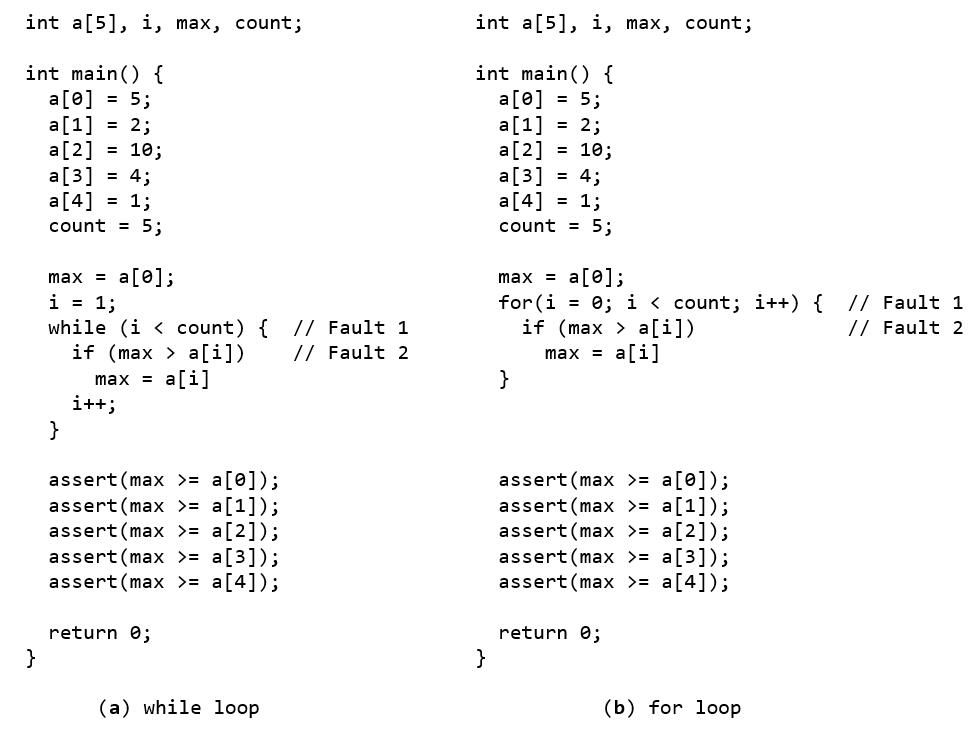
\includegraphics[width=5in]{img/Fig5-1.jpg}
\caption{While loop and for loop faulty programs}
\label{fig:WaF}
\end{figure}

\subsubsection{Experimental Results}
% 对while和for循环的两个错误版本中只需要采用一个测试用例便可以得到修复的结果
For loop statement fault, one test case is sufficient for finding the repairing statement.
The results are listed in table \ref{table:RoCTC}. Meanings of columns in table \ref{table:RoCTC} are listed below:

\begin{enumerate}
\item {\it Version}: the version number of the corresponding version.
\item $V$             : the number of global and relevant boolean variables.
\item $LoBP_{1}$      : the length of converted boolean program when five test cases are introduced.
\item $Time_{1}$($s$) : the time in seconds used to repair the given boolean program when five test cases are introduced.
\item $Result_{1}$    : the percentage of passed tests among the given 2000 tests when five test cases are introduced.
\item $LoBP_{2}$      : the average length of converted boolean program when multiple test cases are introduced.
\item $Time_{2}$($s$) : the time in seconds used to repair the given boolean program when multiple test cases are introduced.
\item $Result_{2}$    : the number of test cases which cover bad routes effectively and the total number of test cases we use.
\end{enumerate}

\begin{table}
\small
\center
\caption{Results of Customized Test Cases}
\label{table:RoCTC}
\begin{tabular}{|c|c|c|c|c|c|c|c|}
\hline
Version   & $V$     & $LoBP_{1}$ & $Time_{1}$($s$) & $Result_{1}$ &$LoBP_{2}$ & $Time_{2}$($s$) & $Result_{2}$ \\
\hline
$while_1$ & $4/40$  & $177$      & $0.38$          & $89.6\%$     & $177$     & $14.1$          & $10/100$     \\
\hline
$while_2$ & $5/40$  & $178$      & $0.31$          & $58.3\%$     & $178$     & $2.7$           & $2/100$      \\
\hline
$for_1$   & $4/40$  & $177$      & $0.26$          & $89.6\%$     & $177$     & $14$            & $10/100$     \\
\hline
$for_2$   & $5/40$  & $178$      & $0.30$          & $58.3\%$     & $178$     & $2.9$           & $2/100$      \\
\hline
\end{tabular}
\end{table}

% 从实验结果可以看出对于包含while和for循环结构的程序的循环控制条件语句错误以及if控制条件语句错误,本文所设计的布尔程序修复逆向转换工具也能对其进行修复,进一步验证了本文所设计工具的有效性。
Judging from the experimental results, the tool is capable of handling loop statement fault and conditional control flow statement fault, which also provides convincing evidence of the tool's effectiveness.

% 在附录一中将会给出本章实验的具体测试用例的错误语句、布尔程序修复语句以及转换后的修复结果语句。
% TODO 添加附录引用
In Appendix A, the concrete test cases we used in the experiment and the respective boolean repairs and converted $C$ repairing statements will be listed respectively.

\subsection{Conclusions}
% 本章的实验结果数据表明本文的方法对于控制条件错误和赋值语句右部错误例如赋值逻辑错误、操作符错误、返回语句错误等程序里实际存在的错误能够给出实际有效且符合坃程序语法语义的修复结果。
Based on the experimental results listed in the former sections, one can say the tool is capable of producing an effective and intuitive repair statement for many kinds of faults, including assignment statement fault and conditional control flow statement fault, which generally exist in most faulty programs.

% Griesmayer[18]在2005年的工作自动找到布尔程序的修复结果之后需要通过程序员人工地将结果转换为布尔程序的结果,没有达到自动化的目的。
In 2005, Griesmayer managed to find the boolean repair automatically\cite{RoBPwaAtC}, but manual intervene is still needed to convert the boolean repair back to the original programming language. In this sense, Griesmayer's work failed to achieve complete automation for program repair.
% 实验结果表明本文的工作完成了程序修复的自动化过程,能够直接地找到坃程序的有效修复。
Judging from the experimental results, our tool is capable of completing the whole process of program repair automatically and producing an effective repair statement.

% Weimer[22]在2009年提出的利用遗传算法来进行程序修复的方法修复的是死循环和段错误以及堆栈溢出等错误类型,并没有实验结果显示能够修复具体的赋值逻辑错误和操作符错误等。
In 2009,  Forrest and Weimer for the first time apply evolutionary computation to repair a real-world software system\cite{AFPUGP}. Their repairing system was capable of repairing faults like
infinite loop and stack overflow, but there was no experimental result that proved their tool supports assignment fault or control flow fault.
% 本文能够修复的错误类型更多的是程序语句逻辑上的错误,与Weimer等人解决的问题领域有差别。
The fault model we discussed in this paper focuses on logical faults of program statements, which makes a difference from Weimer's study.
